\documentclass[10pt,a4paper,twocolumn]{article}

\input{pisika.dat}

%  Editorial staff will uncomment the next line
% \input{staff.hed}


\begin{document}

%--------------------------------------------------------------------------
%  fill in the paper's title, author(s), and corresponding institutions
%--------------------------------------------------------------------------
\providecommand{\ShortAuthorList}[0]{Alžběta Prášilová}
\title{Modelování chování chemotaktických buněk v bludištích}
\author[1,*]{Alžběta Prášilová}
\affil[1]{Přírodovědecká fakulta Univerzity Karlovy, Bioinformatika, Praha, Česká republika}
\affil[*]{alzbeta.prasilova@seznam.cz}

\date{\dateline{}}

\begin{abstract}
\noindent
%---------------------------------------------------------------------------
%               Include abstract and keywords here
%---------------------------------------------------------------------------
Buňky potřebují migrovat přes dlouhé vzdálenosti, používají na to proces zvaný chemotaxe. Chemotaxe je cílený pohyb buněk reagujících na
gradienty látek v prostředí. Na dlouhé vzdálenosti mohou však být gradienty téměř nedetekovatelné.
Buňky toto překonávají vytvářením lokálních gradientů rozkladem atraktantu. Chemotaxe a samovytvářené gradienty dovolují buňkám
navigovat složité trasy s vysokou účinností. V této práci je představen multiagentní buněčný model simulující rozkládající a nerozkládající buňky v bludištích. Při analýze byla prokázána schopnost modelu simulovat samovytvářené gradienty a výsledky byly konzistentí s článkem Tweedy et al., 2020\textsuperscript{\cite{h-model}}.



\DOI{} % do not delete this line
\end{abstract}

\maketitle
\thispagestyle{titlestyle}



%---------------------------------------------------------------------------
%               the main text of your paper begins here
%---------------------------------------------------------------------------
\section{Úvod}

Buňky potřebují migrovat přes dlouhé vzdálenosti, jak už během běžného
embryonálního vývoje, tak i v průběhu onemocnění. Úspěšně navigují složitými a
větvenými cestami, kterými by samy od sebe nebyly schopny projít. Na to využívají
proces zvaný chemotaxe. Chemotaxe je cílený pohyb buněk reagujících na
gradienty látek v prostředí. Příkladem buněk používajících chemotaxi k pohybu
jsou například neutrofily extravazující do infikované tkáně, zárodečné buňky
migrující embryonální dermis či metastáze glioblastomu skrz bílou hmotu mozku.
Chemotaktické buňky detekují gradienty atraktantů pomocí rozdílů v obsazenosti
receptorů. Dokážou rozlišit rozdíly o 1 \%, což usnadňuje navigaci na krátké
vzdálenosti. Nicméně, nad 0,5 až 1 mm mohou gradienty být nedetekovatelné.
Buňky toto překonávají vytvářením místních gradientů rozkladem atraktantů, což
zajišťuje účinnou chemotaxi. Samovygenerované gradienty udržují koncentraci
atraktantu na nedonasycené úrovni a umožňují buňkám pružně a přesně reagovat
na změny gradientu a směřovat svůj pohyb tak, aby dosáhly požadovaného cíle či
místa.


\section{Matematický model}
V této práci je představen matematický model, který využívá chemotaxi a samo-vytvářené gradienty atraktantu pro simulaci chování buněk. Na základě již existujícího modelu, (\emph{H-model})\textsuperscript{\cite{h-model}} 
byly přizpůsobeny a konfigurovány parametry a funkce%(?procesy/mechanismy,..)
, aby lépe odpovídaly konkrétním výzkumným cílům. Tato adaptace umožňuje zkoumat rozdíly v dynamice pohybu buněk využívajích samovygenerované gradienty a má za cíl otestovat hypotézu, že buňky tohoto typu jsou v navigaci prostorem úspěšnější než-li ty, co tak nečiní. Úpravou a adaptací modelu na tuto problematiku lze získat zajímavé  poznatky o jeho bližším fungování a získat hlubší porozumění o chování buněk za různých podmínek chemotaxe. Podrobnější popis modelu
je k nahlédnutí v části \ref{subsec:model_setup}.



\section{Výsledky}

První část analýzy modelu spočívala v optimalizaci parametrů, jež je podrobněji popsána v části \ref{subsec:parameter_choice}.
Další část experimentů měla za cíl otestovat hypotézu\textsuperscript{\cite{tweedy2020}}, že buňky rozkládající atraktant a tím si vytvářející lokální gradient, nacházejí v bludišti zdroj atraktantu rychleji  než ty, co ho nerozkládají. 
V experimentech byla použita jako metrika k ohodnocení rychlosti počet kroků simulace, za který došla buňka až ke zdrojové buňce vypouštěící atraktant. Jejich setkání bylo v modelu sprostředkováno pomocí reakce jejich receptorů a následné změny stavu zdrojové buňky.

\subsection{Varianty labyrintů}
\label{subsec:lab_variants}
Pro analýzu modelu a otestování hypotézy byla zvolena 3 různá bludiště.
První a nejjednodušší struktura bludiště (viz obrázek \ref{fig:snake_maze}, označena jako \texttt{snake\_maze}, byla z části použita i pro optimalizaci parametrů. 
Druhý typ labyrintů (viz obrázek \ref{fig:round_maze}) byl označen jako \texttt{round\_maze}, je podstatně složitější než \texttt{snak\_maze} a vyznačuje se tím, že zdrojová buňka je v něm umístěna doprostřed.
Poslední experiment byl proveden v bludišti označeném jako \texttt{square\_maze} (viz obrázek \ref{fig:square_maze}).


\begin{figure}[tb]
  \centering
  
\includegraphics[width=0.98\linewidth]{images/snake_maze.png}
  \caption{\textbf{Nejjednodušší struktura:} 
  Tvar nejjednoduššího bludiště použitý k prvnímu experimentu, označen jako \texttt{snake\_maze}.}
  \label{fig:snake_maze}
\end{figure} 

\begin{figure}[tb]
  \centering
  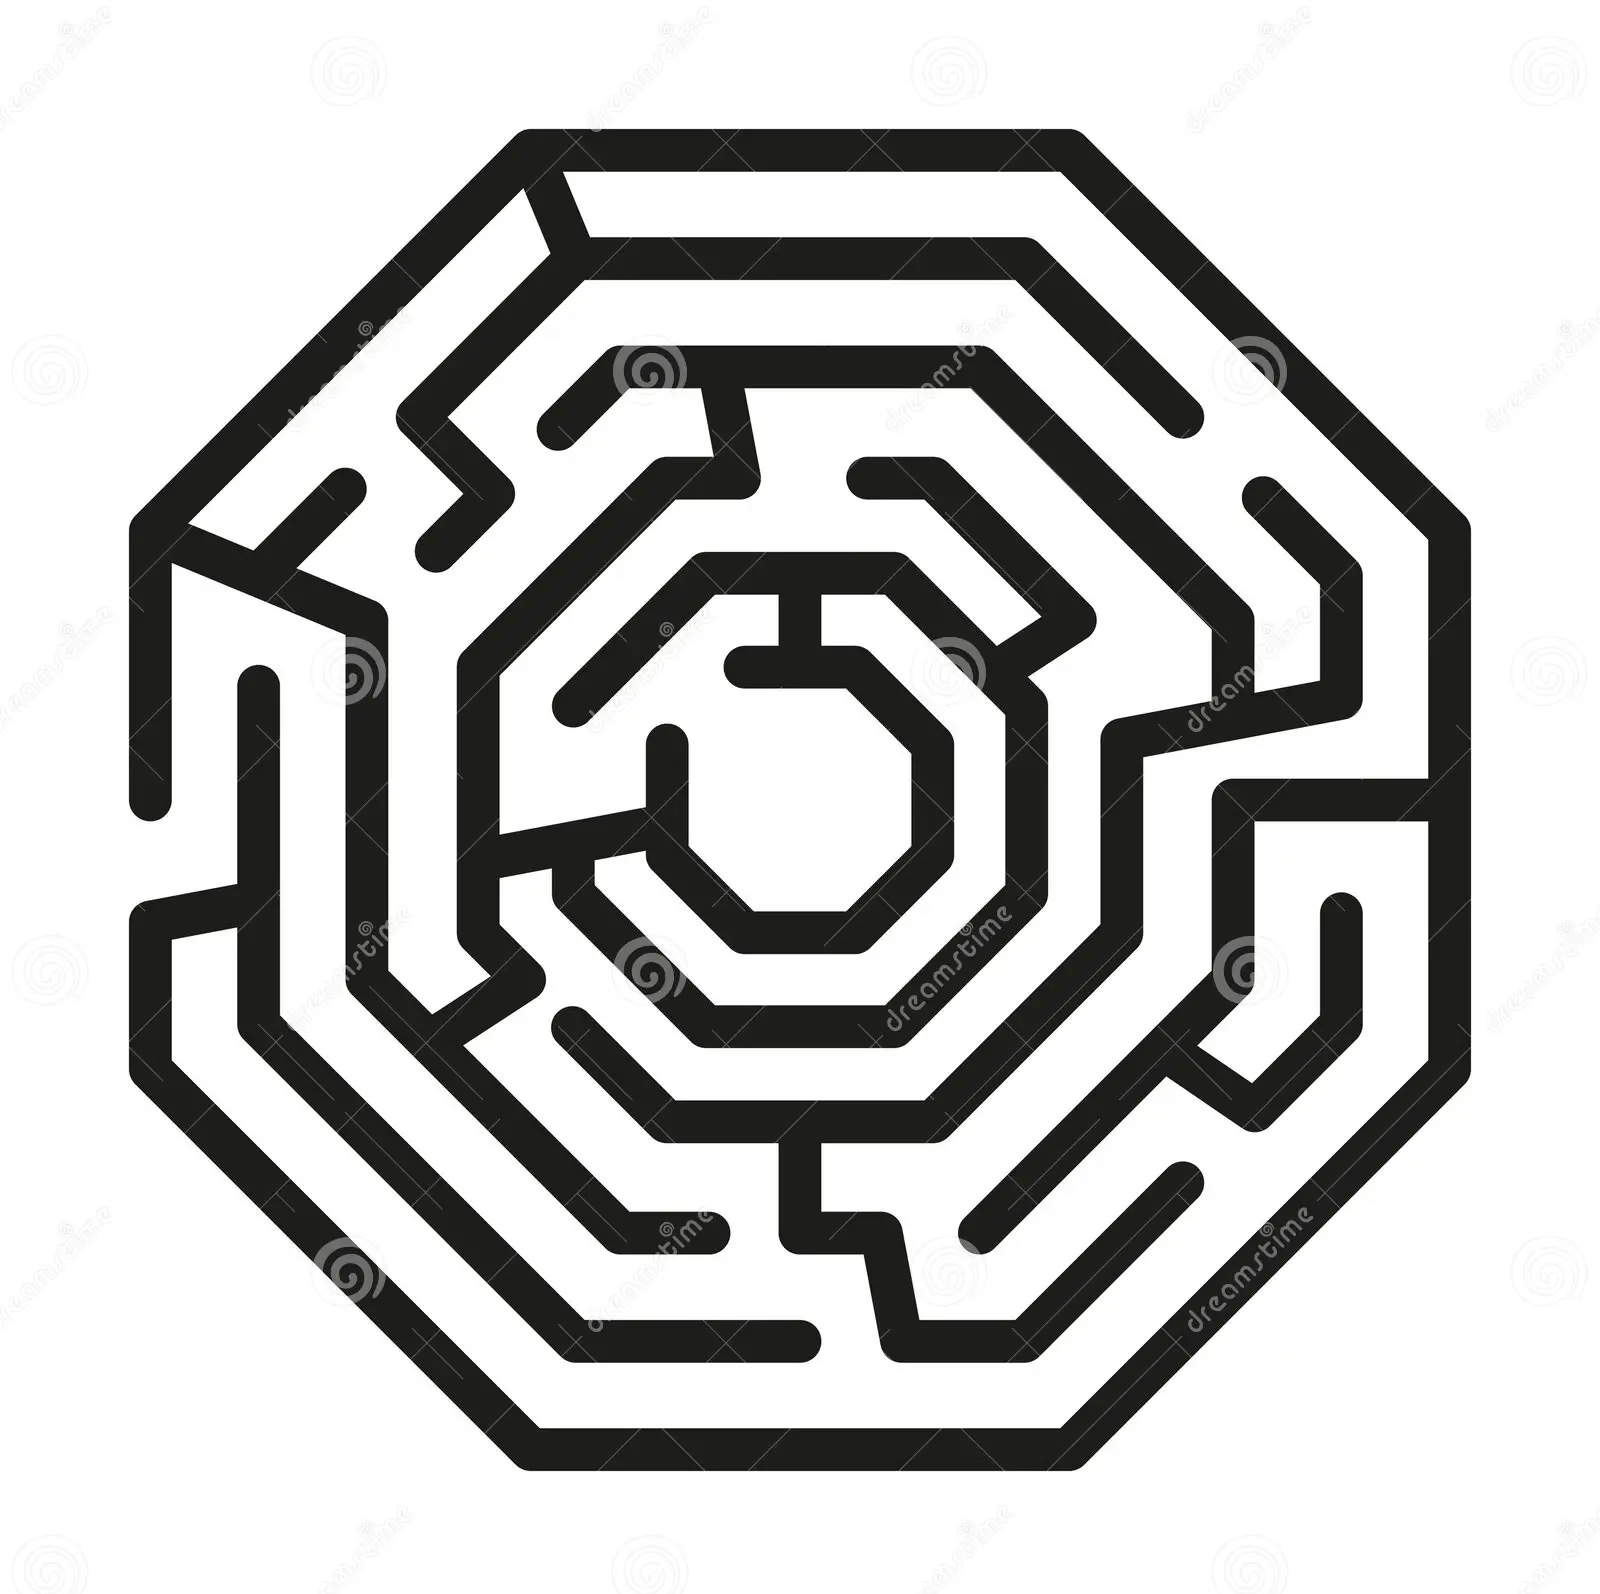
\includegraphics[width=0.98\linewidth]{images/round_maze.png}
  \caption{\textbf{Druhý typ labyrintu:} 
  Druhý typ labyrintu se zdrojovou buňkou uprostřed, označen jako \texttt{round\_maze}\textsuperscript{\cite{round_maze}}.}
  \label{fig:round_maze}
\end{figure} 

\begin{figure}[tb]
  \centering
  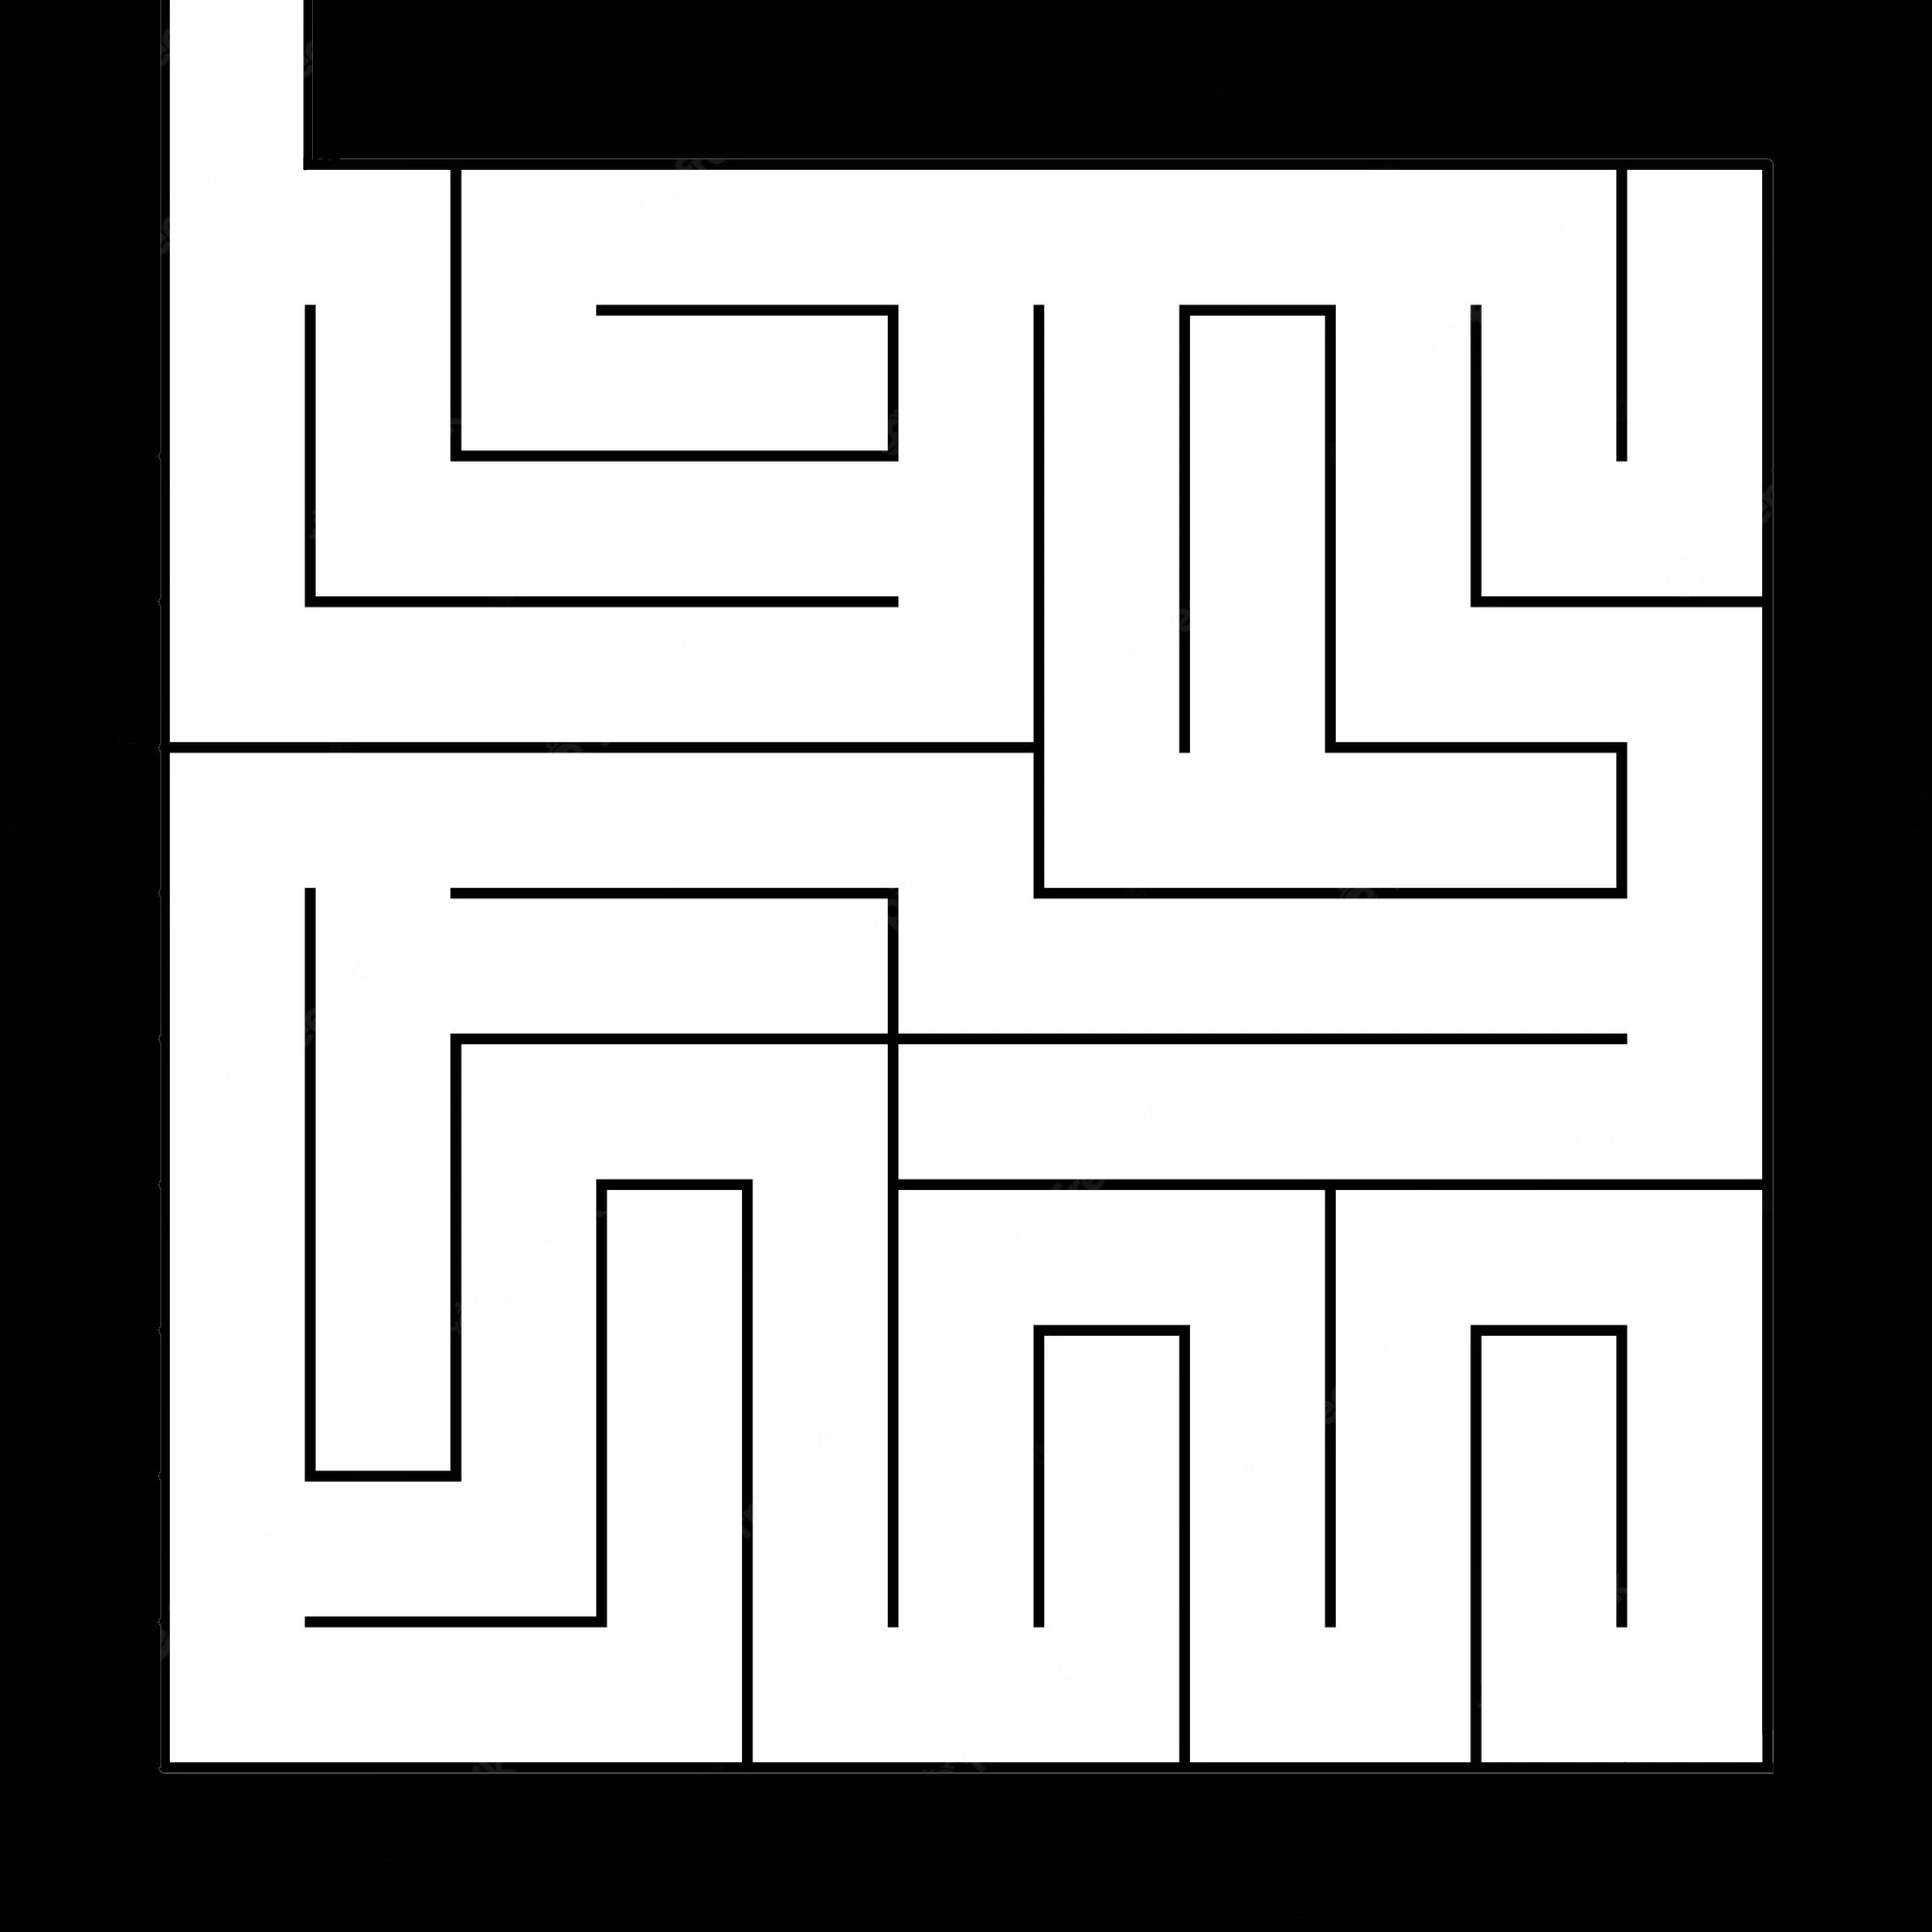
\includegraphics[width=0.98\linewidth]{images/square_maze.png}
  \caption{\textbf{Třetí typ labyrintu:} 
  Struktura třetího typu bludiště, označen jako \texttt{square\_maze}\textsuperscript{\cite{square_maze}}.}
  \label{fig:square_maze}
\end{figure} 





\subsection{Experimenty}
\label{subsec:variant_comparision}

První experiment proběhl v \texttt{snake\_maze}. V rámci dodatečné optimalizace parametru množství vypuštěné látky buňkou do prostředí (parametr $prod\_v$, viz tabulka \ref{table:parametry}) byla analýza prováděna pro 130 simulací. Model byl u \texttt{snake\_maze} velmi citlivý na změny parametrů a obecně výsledky prvního experimentu se zdají být více či méně nejednoznačné. Podrobnější výsledky a přesné nastavení při dodatečné optimalizaci parametrů je dostupné v githubovém repositáři\textsuperscript{\cite{self_gen_gradient}}. Zprůměrované výsledky všech simulací v \texttt{snake\_maze} s různými parametry jsou zobrazeny pomocí boxplotu na obrázku \ref{fig:snake_all}. Boxplot pro 20 simulací se stejnými parametry (viz sekce \ref{subsec:experiment_description}) jako ostatní experimenty je na obrázku \ref{fig:snake}. Příklad vizualizace simulace v \texttt{snake\_maze} je vidět na obrázku \ref{fig:snake_vis}. 

Druhý experiment byl prováděn v \texttt{round\_maze}. Bylo spuštěno celkem 20 simulací, jejichž výsledky jsou zobrazeny pomocí boxplotu na obrázku \ref{fig:round}. Z boxplotu je vidět, že buňky rozkládající atraktant došly ke zdrojové buňce dříve než ty, co ho nerozkládají. Příklad vizualizace simulace v \texttt{snake\_maze} je vidět na obrázku \ref{fig:round_vis}. 

Poslední bludiště bylo \texttt{square\_maze}. Simulace byla spuštěna celkem 20krát. výsledky z \texttt{square\_maze} jsou pomocí boxplotu zobrazeny na obrázku \ref{fig:square}. Výsledky simulací jsou konzistentní s článkem Tweedy et al., 2020\textsuperscript{\cite{tweedy2020}} a potvrzují hypotézu, že buňky rozkládající atraktant navigují prostorem lépe než buňky, co ho nerozkládají. Příklad vizualizace simulace v \texttt{snake\_maze} je vidět na obrázku \ref{fig:square_vis}. 


\begin{figure}[tb]
  \centering
  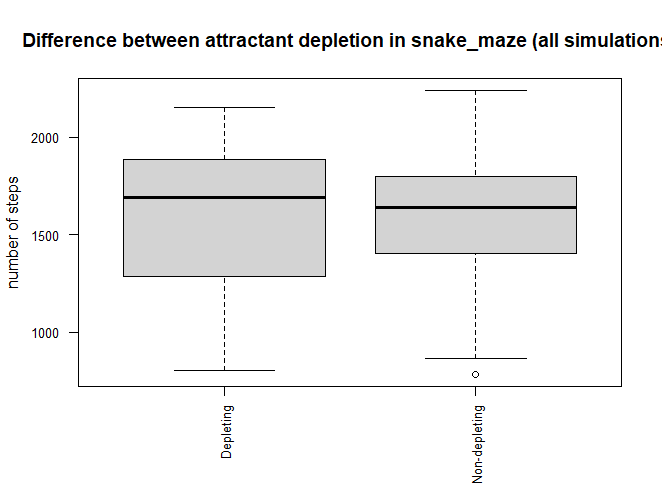
\includegraphics[width=0.98\linewidth]{images/snake_all.png}
  \caption{\textbf{Výsledky všech simulací v \texttt{snake\_maze}:} 
  Boxplot zobrazující výsledky všech simulací prováděných v \texttt{snake\_maze}. Výsledky jsou nekonzistentní s hypotézou z článku Tweedy et al., 2020\textsuperscript{\cite{tweedy2020}}.}
  \label{fig:snake_all}
\end{figure} 

\begin{figure}[tb]
  \centering
  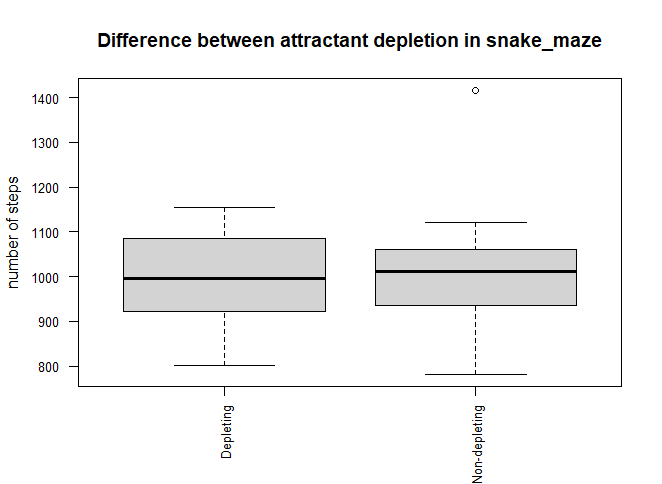
\includegraphics[width=0.98\linewidth]{images/snake.png}
  \caption{\textbf{Výsledky simulací v \texttt{snake\_maze}:} 
  Boxplot zobrazující výsledky simulací prováděných v \texttt{snake\_maze} se pevně danými parametry popsanými v sekci \ref{subsec:experiment_description}. Výsledky jsou však nekonzistentní s hypotézou z článku Tweedy et al., 2020\textsuperscript{\cite{tweedy2020}}.}
  \label{fig:snake}
\end{figure} 

\begin{figure}[tb]
  \centering
  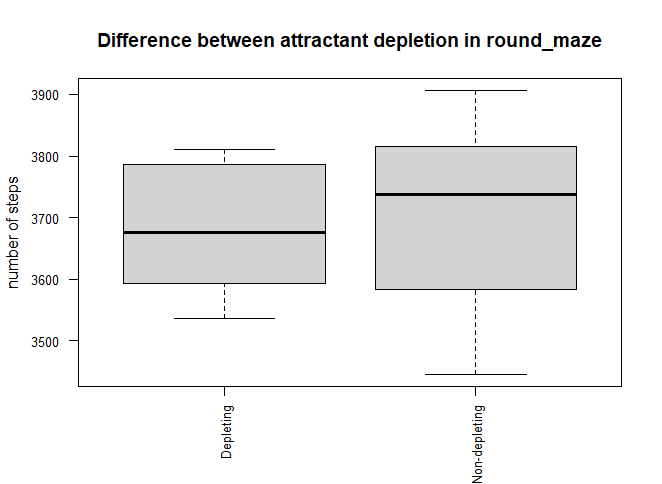
\includegraphics[width=0.98\linewidth]{images/round.png}
  \caption{\textbf{Výsledky simulací v \texttt{round\_maze}:} 
  Simulace v \texttt{round\_maze} se zdrojovou buňkou uprostřed přinesly výsledky konzistentní s článkem Tweedy et al., 2020\textsuperscript{\cite{tweedy2020}}.}
  \label{fig:round}
\end{figure} 

\begin{figure}[tb]
  \centering
  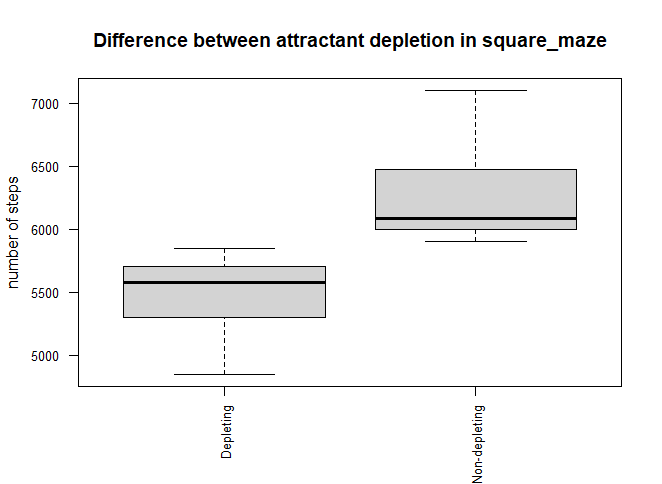
\includegraphics[width=0.98\linewidth]{images/square.png}
  \caption{\textbf{Výsledky simulací v \texttt{square\_maze}:} 
  Simulace v \texttt{square\_maze} přinesly výsledky konzistentní s článkem Tweedy et al., 2020\textsuperscript{\cite{tweedy2020}}, tedy buňky rozkládající atraktant se ke zdrojové buňce dostaly dříve než ty, co ho nerozkládají.}
  \label{fig:square}
\end{figure} 

\begin{figure}[tb]
  \centering
  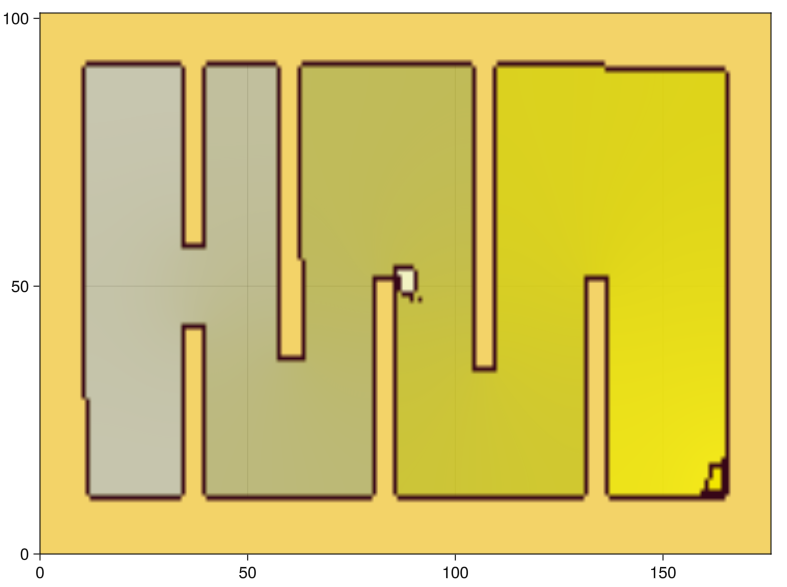
\includegraphics[width=0.98\linewidth]{images/snake_visual.png}
  \caption{\textbf{Příklad simulace v \texttt{snake\_maze}:} 
  Příklad vizuální formy simulace v \texttt{snake\_maze}.}
  \label{fig:snake_vis}
\end{figure} 

\begin{figure}[tb]
  \centering
  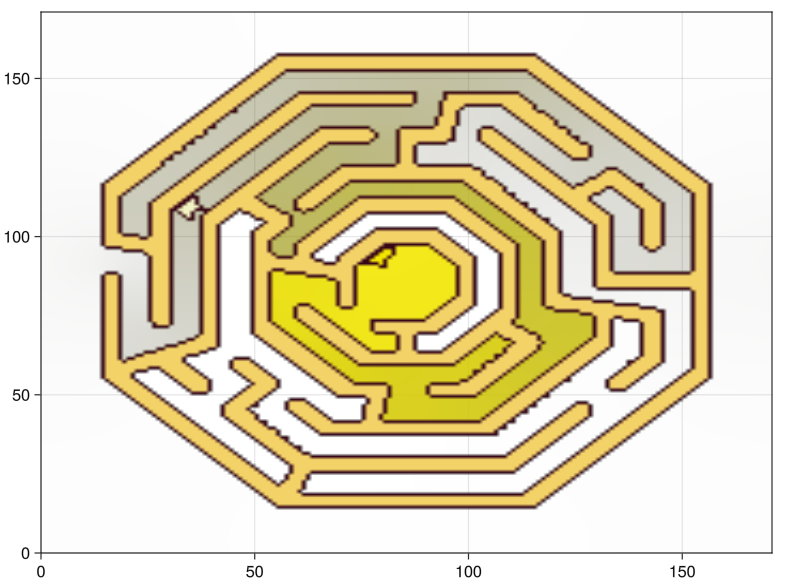
\includegraphics[width=0.98\linewidth]{images/round_visual.png}
  \caption{\textbf{Příklad simulace v \texttt{round\_maze}:} 
  Příklad vizuální formy simulace v \texttt{round\_maze}.}
  \label{fig:round_vis}
\end{figure} 

\begin{figure}[tb]
  \centering
  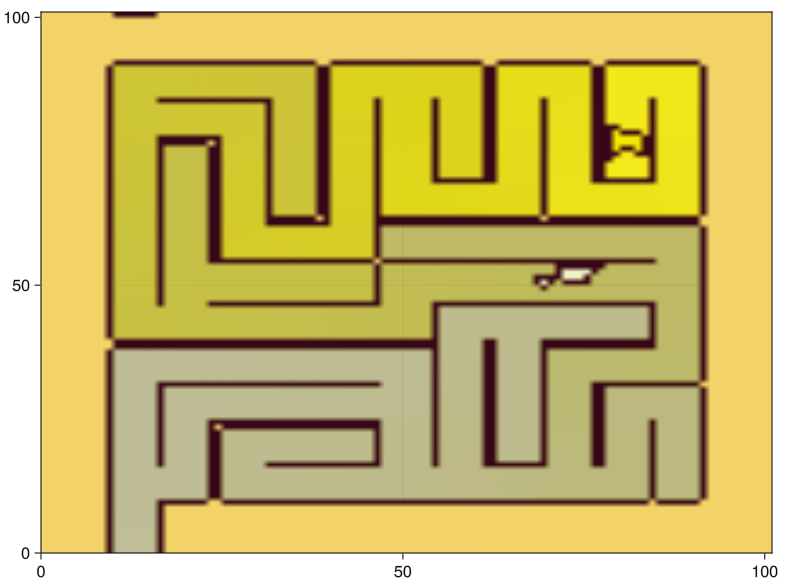
\includegraphics[width=0.98\linewidth]{images/square_visual.png}
  \caption{\textbf{Příklad simulace v \texttt{square\_maze}:} 
  Příklad vizuální formy simulace v \texttt{square\_maze}.}
  \label{fig:square_vis}
\end{figure} 


\section{Diskuze}
Navržený model dokázal ve většině případů potvrdit hypotézu\textsuperscript{\cite{tweedy2020}}, že buňky rozkládající atraktant a tím si vytvářející lokální gradient, nacházejí v bludišti zdroj atraktantu rychleji  než ty, co ho nerozkládají. 
Ukázalo se, že u složitějších labyrintů byl rozdíl v rychlosti jednoznačný, načež u jednoduššího designu bludiště byl model velmi citlivý na změny parametrů a výsledky byly nejednoznačné až vyvracející výsledky článku Tweedy et al., 2020\textsuperscript{\cite{tweedy2020}}. Tento výsledek může mít několik vysvětlení, může poukazovat na potenciálně nekonzistentní implementaci chemotaxe v \textit{H-modelu}, ne kompletně správné a obecně aplikovatelné výsledky článku Tweedy et al., 2020\textsuperscript{\cite{tweedy2020}} nebo pravděpodobně nedostatečné prozkoumání prostoru parametrů a jejich neoptimální výběr. Prošetření tohoto problému by mohlo být zajímavé do dalších prací.  

\section{Metody}

\subsection{Popis modelu}
\label{subsec:model_setup}
Model je adaptací a konfigurací existujícího \textit{H-modelu}\textsuperscript{\cite{h-model}} (popsán v sekci \ref{subsubsec:H-model}) implementovaného pomocí celulárního Pottsova modelu (CPM). CPM je model používaný ve výpočetní biologii a fyzice k simulaci chování a dynamiky buněk a tkání. Je zvláště užitečný pro modelování procesů, jako je migrace buněk, buněčná adheze a vývoj tkání. CPM využívá přístup založený na použití mřížky k reprezentaci biologického systému. Buňky nebo buněčné komponenty jsou obvykle reprezentovány spojenými soubory bodů v mřížce.

\subsubsection{Reprezentace mřížky} Každý bod mřížky odpovídá základní jednotce prostoru. Mřížka může být 2D nebo 3D, v závislosti na povaze modelovaného systému.

\subsubsection{Energie a Hamiltonian} CPM používá energetický přístup k modelování buněčného chování. Každé konfiguraci systému je přiřazena energie, Hamiltonian (\textit{H}) na základě interakcí a vlastností, jako je buněčná adheze, adheze buňky k substrátu a omezení objemu buňky. \textit{H} reprezentuje celkovou energii systému.

\subsubsection{Buňky} Buňky jsou charakterizovány parametry, jako je adheze buněk, objem buňky, povrchová plocha a další. Tyto parametry ovlivňují chování buněk v rámci modelu. Buňky mohou migrovat, měnit tvar, slučovat se nebo se dělit na základě \textit{H} a příslušných parametrů. Pohyb a chování buněk jsou řízeny minimalizací celkové energie systému.

\subsubsection{H-model}
\label{subsubsec:H-model}
\textit{H-model} je model biologické buňky a mezibuněčných interakcí. Je řízen sadou pravidel popisujících chování buňky v závislosti na aktuálním stavu a blízkém okolí buňky. Přistupuje k buňce jako nediferenciované, tedy zygotické, schopné přecházet ze stavů do stavů na základě jejího chování a okolí.

\paragraph{Zygotický graf} popisuje dění uvnitř buňky. Je to multigraf a skládá se z tzv. produkčního, pohybového, receptorového a apoptotyckého grafu. Grafy dohromady shrnují pravidla v přecházení buněk mezi stavy. Tzv. \textit{kumulační stav} popisuje a kvantifikuje aktuální stav buňky.

\paragraph{Konfigurace modelu} je prováděna pomocí konfiguračních souborů. Obsahuje 4 hlavní sekce, které jsou popsány v tabulce \ref{table:sekce}.


\begin{table}[t]
  \centering % center-align tables within a column
  \begin{tabular}{l p{5cm}}
  \toprule
  Sekce & Popis \\
  \midrule
    \texttt{:vaxes} & Definice látek figurujících v modelu(atraktant, receptory,...)). \\
    \texttt{:reactions} & Reakce a jejich pravidla (reakce mezi receptory, reakce receptoru na látku)\\
    \texttt{:cells} & Definice buněk v modelu\\	
    \texttt{:rule\_graph} & Popis zygotického grafu\\	
    
  \bottomrule
  \end{tabular}
  \caption{Seznam a popis sekcí konfiguračního souboru k \textit{H-modelu}.} \label{table:sekce} 
\end{table}

\subsubsection{Vlastní adaptace H-modelu}
V této práci byl \textit{H-model} přizpůsoben ke zkoumání chování chemotaktických buněk a pozorování rozdílů mezi buňkami rozkládající atraktant a těmi, co tak nečiní. Experimenty byly prováděny v bludištích a uzavřených prostředích, bylo tedy nutné vytvořit definici nepropustné bariéry a způsob jak definovat tvar bludiště. Byla vytvořena funkce, která z načteného obrázku bludiště vyfiltrovala černé pixely a převedla je v nepropustnou bariéru v modelu. Pro jednotlivé experimenty byly použity 2 typy buněk - \textit{rozkládající} a \textit{nerozkládající}. Hlavní konfigurace modelu byla v rámci optimalizace a výběru parametrů, popsaného v sekci \ref{subsec:parameter_choice}.


\subsection{Analýza modelu}

Veškeré zdrojové kódy implementace modelu a analýzy výsledků společně s
výsledky experimentů a jejich podrobným nastavením jsou k nahlédnutí v 
githubovém repozitáři\textsuperscript{\cite{github_repo}}.
Model je 
naimplementován v jazyce Julia, v němž je naimplementován
také zdrojový kód pro běh experimentů.
Výsledky byly analyzovány za pomoci jazyka R v prostředí 
R-Studio.

\begin{table}[t]
  \centering % center-align tables within a column
  \begin{tabular}{l p{4cm}}
  \toprule
  Parametr & Popis \\
  \midrule
    $vaxes\_rule\_step \in \mathbb{N}$ & Šíření látek v protředí za jeden krok simulace
    \\ 
    $k \in (0, 1)$ & Reakční konstanta rozkladu atraktantu \\
    $r \in \mathbb{N}_0$ & Počet receptorů na rozklad atraktantu\\
    $D \in (0, 1)$ & Koeficient difuze atraktantu\\
    $prod\_v \in \mathbb{N}_0$ & Množství látky produkované buňkou do prostoru za jeden krok simulace \\
  \bottomrule
  \end{tabular}
  \caption{Seznam zkoumaných parametrů modelu.} \label{table:parametry} 
\end{table}

\subsection{Výběr parametrů}
\label{subsec:parameter_choice}
V rámci zkoumání a optimalizace parametrů byly vybrány pouze některé parametry, na které byl model experimentálně nejcitlivější.
(viz. tabulka \ref{table:parametry}). Pro experimenty ve složitějších bludištích byly parametry vybrány. Pro ohodnocení kvality volby
parametrů byl použit jako metrika počet kroků za který doputuje buňka ke zdroji atraktantu \texttt{var-0} (viz. část \ref{subsec:map_variants}). 
Byl zkoumán vliv rychlosti šíření látek v prostředí za jeden krok simulace (parametr $vaxes\_rule\_step$), 
reakční konstanta rozkladu atraktantu (parametr $k$), počet receptorů na rozklad atraktantu (parametr $r$), koeficient difuze atraktantu (parametr $D$) a množství látky produkované buňkou do prostoru za jeden krok simulace (parametr $prod\_v$), viz tabulka \ref{table:parametry}. 


Pro každý z vybraných parametrů byla provedena analýza, která zahrnovala průzkum chování modelu a jeho ohodnocení výše popsanou metrikou. Vyhodnocení analýzy je znázorněno pomocí grafů \ref{fig:vrs}, 
\ref{fig:k}, \ref{fig:r}, \ref{fig:D} a \ref{fig:prod_v}.

\begin{figure}[tb]
  \centering
  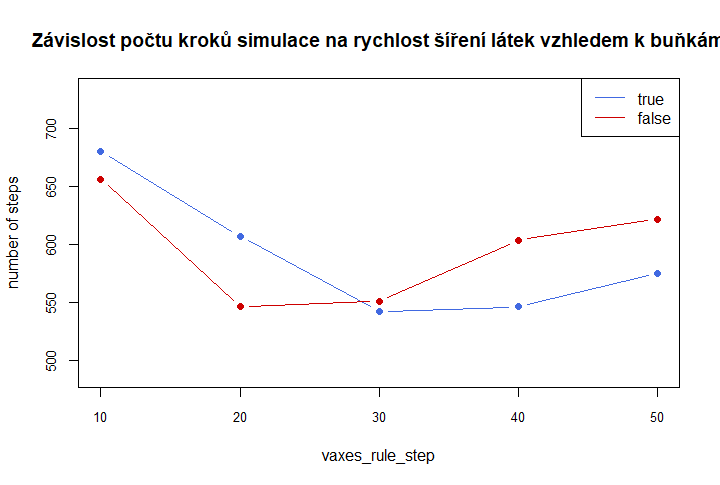
\includegraphics[width=0.9\linewidth]{images/vrs.png}
  \caption{\textbf{Počet kroků simulace v závislosti na parametru `vaxes\_rule\_step`:}
  Počet kroků simulace je nižší pro buňky rozkládající atraktant (\textit{true}) než pro ty, co tak nečiní (\textit{false}), když je rychlost šíření látky za 1 krok simulace (paramter $vaxes\_rule\_step$) větší nebo rovno $30$.}
  \label{fig:vrs}
\end{figure}

\begin{figure}[tb]
  \centering
  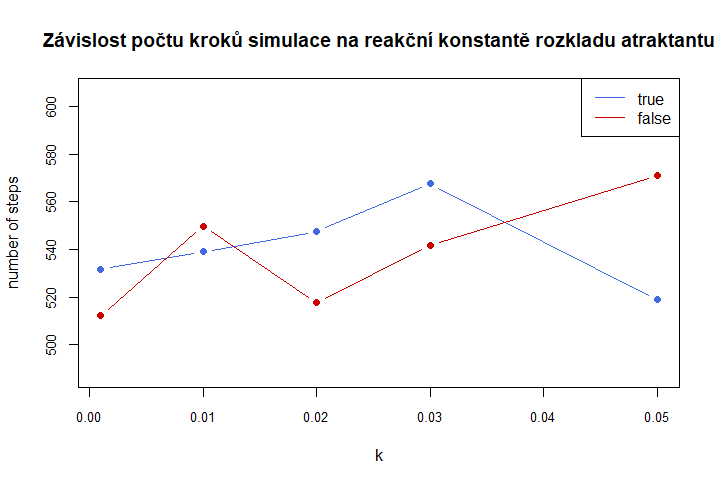
\includegraphics[width=0.9\linewidth]{images/k.png}
  \caption{\textbf{Počet kroků simulace v závislosti na parametru `k`:}
  Počet kroků simulace je nižší pro buňky rozkládající atraktant (\textit{true}) než pro ty, co tak nečiní (\textit{false}), když je v rozmezí $(0.001,0.5)$ reakční konstanta rozkladu atraktantu (parametr $k$) rovna $0.01$ nebo $0.5$.}
  \label{fig:k}
\end{figure}

\begin{figure}[tb]
  \centering
  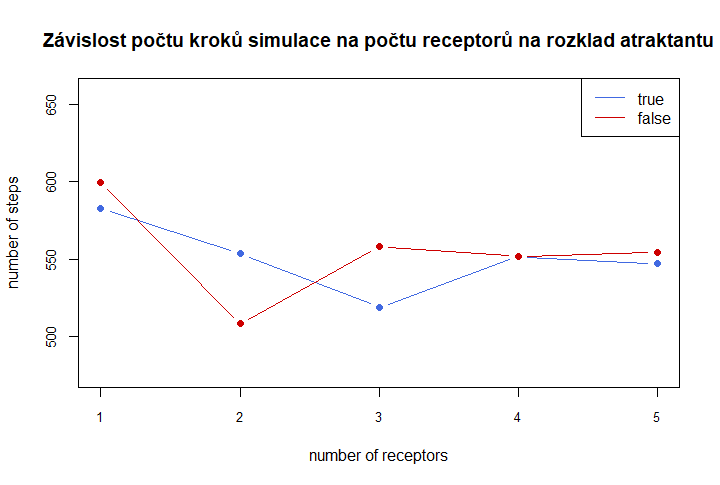
\includegraphics[width=0.9\linewidth]{images/num_rec.png}
  \caption{\textbf{Počet kroků simulace v závislosti na parametru `r`:}
  Počet kroků simulace je nižší pro buňky rozkládající atraktant (\textit{true}) než pro ty, co tak nečiní (\textit{false}), když je v rozmezí $(1,5)$ počet receptorů na rozklad atraktantu (parametr $r$) roven $1, 3$ nebo $5$.}
  \label{fig:r}
\end{figure}

\begin{figure}[tb]
  \centering
  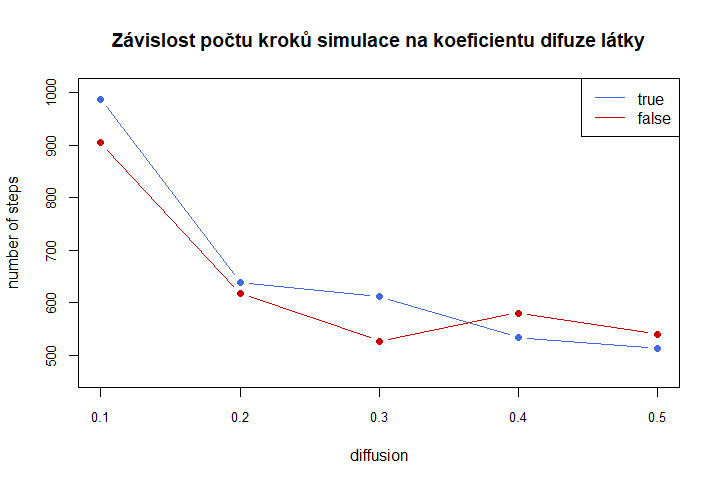
\includegraphics[width=0.9\linewidth]{images/difuze.png}
  \caption{\textbf{Počet kroků simulace v závislosti na parametru `D`:}
  Počet kroků simulace (PKS) klesá s rostoucím koeficientem difuze (parameter $D$). PKS je nižší pro buňky rozkládající atraktant (\textit{true}) než pro ty, co tak nečiní (\textit{false}), když je difuzní koeficient (parametr $r$) větší nebo roven $0.4$.}
  \label{fig:D}
\end{figure}

\begin{figure}[tb]
  \centering
  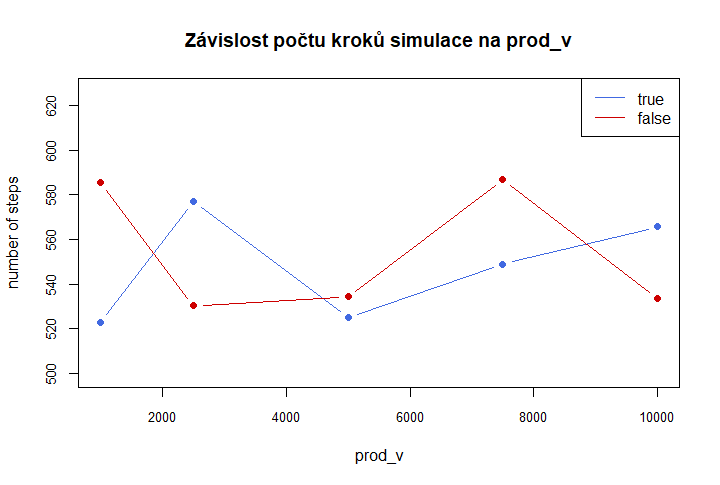
\includegraphics[width=0.9\linewidth]{images/prod_v.png}
  \caption{\textbf{Počet kroků simulace v závislosti na parametru `prod\_v`:}
  Počet kroků simulace je nižší pro buňky rozkládající atraktant (\textit{true}) než pro ty, co tak nečiní (\textit{false}), když je v rozmezí $(1000,10000)$ množství látky produkované buňkou do prostoru (parametr $prod\_v$) roven $1000, 5000$ nebo $7500$.}
  \label{fig:prod_v}
\end{figure}



\subsection{Popis experimentů}
\label{subsec:experiment_description} 
Hlavní část experimentů byla zaměřena na potvrzení hypotézy \textsuperscript{\cite{tweedy2020}}, že buňky rozkládající atraktant a tím si vytvářející lokální gradient, nacházejí v bludišti zdroj atraktantu rychleji  než ty, co ho nerozkládají. 
Experiment používal k ohodnocení rychlosti počet kroků simulace, za který došla buňka až ke zdrojové buňce vypouštěící atraktant. Na základě optimalizace parametrů
(viz. část \ref{subsec:parameter_choice}) a předchozí zkušenosti, byly pro experimenty v bludištích pevně zvoleny následující hodnoty  parametrů:

\begin{itemize}
  \item $vaxes\_rule\_step = 50$
  \item $k = 0.01$
  \item $r = 3$
  \item $D = 0.4$
  \item $prod\_v = 10000$
\end{itemize}


% Please use pisikabst.bst. You may your own *.bib file.
\clearpage
\bibliographystyle{pisikabst}
\bibliography{bibfile}

\section*{Doplňkové materiály}
Elektronická verze práce obsahuje doplňové materiály obsahující
animace simulací. Elektronická verze práce je dostupná na adrese
\url{https://github.com/prasilal/self_gen_gradient_model.git}


\end{document}